\begin{comment}
\begin{tikzpicture}
\begin{axis}[height=0.40\textheight,width=0.40\textwidth,style={font=\footnotesize},grid=major,grid style={dotted},align=center,xlabel={Kontraktionsmodus},ylabel={Tensorstufe},title={TLib-SB-P3},scaled ticks=false,zticklabel=\pgfmathprintnumber{\tick},zlabel={Durchsatz [Gflops/s]},view={-45}{45}]
\addplot3[surf]
coordinates{(1.000,2.000,31.469) (1.000,3.000,33.163) (1.000,4.000,32.263) (1.000,5.000,29.593) (1.000,6.000,20.940) (1.000,7.000,14.973) 

(2.000,2.000,25.250) (2.000,3.000,33.379) (2.000,4.000,27.675) (2.000,5.000,16.795) (2.000,6.000,6.767) (2.000,7.000,2.642) 

(3.000,2.000,25.149) (3.000,3.000,29.800) (3.000,4.000,15.624) (3.000,5.000,9.714) (3.000,6.000,4.561) (3.000,7.000,2.271) 

(4.000,2.000,25.149) (4.000,3.000,29.912) (4.000,4.000,28.394) (4.000,5.000,9.238) (4.000,6.000,4.664) (4.000,7.000,2.321) 

(6.000,2.000,25.132) (6.000,3.000,30.192) (6.000,4.000,28.456) (6.000,5.000,26.045) (6.000,6.000,23.997) (6.000,7.000,2.374) 

(7.000,2.000,25.130) (7.000,3.000,30.130) (7.000,4.000,28.421) (7.000,5.000,26.057) (7.000,6.000,23.977) (7.000,7.000,21.721) 

};
\end{axis}
\end{tikzpicture}
\end{comment}
\begin{comment}
\begin{tikzpicture}
\begin{axis}[height=0.40\textheight,width=0.40\textwidth,style={font=\footnotesize},grid=major,grid style={dotted},align=center,xlabel={Kontraktionsmodus},ylabel={Tensorstufe},title={TLib-SB-P3},scaled ticks=false,zticklabel=\pgfmathprintnumber{\tick},zlabel={Durchsatz [Gflops/s]},view={-45}{45}, zlabel={Standardfehler [\%]}]
\addplot3[surf]
coordinates{(1.000,2.000,4.441) (1.000,3.000,2.520) (1.000,4.000,2.634) (1.000,5.000,3.060) (1.000,6.000,28.452) (1.000,7.000,26.349) 

(2.000,2.000,6.053) (2.000,3.000,0.985) (2.000,4.000,18.811) (2.000,5.000,39.610) (2.000,6.000,27.938) (2.000,7.000,21.212) 

(3.000,2.000,5.745) (3.000,3.000,5.137) (3.000,4.000,26.800) (3.000,5.000,48.648) (3.000,6.000,22.074) (3.000,7.000,18.510) 

(4.000,2.000,5.487) (4.000,3.000,4.115) (4.000,4.000,2.842) (4.000,5.000,40.928) (4.000,6.000,22.946) (4.000,7.000,19.327) 

(6.000,2.000,5.863) (6.000,3.000,3.862) (6.000,4.000,2.371) (6.000,5.000,2.221) (6.000,6.000,2.934) (6.000,7.000,17.326) 

(7.000,2.000,5.673) (7.000,3.000,4.094) (7.000,4.000,2.764) (7.000,5.000,2.195) (7.000,6.000,3.317) (7.000,7.000,5.037) 

};
\end{axis}
\end{tikzpicture}
\end{comment}
%\begin{tikzpicture}
%\begin{axis}[height=0.40\textheight,width=0.40\textwidth,style={font=\footnotesize},grid=major,grid style={dotted},align=center,xlabel={Kontraktionsmodus},ylabel={Tensorstufe},title={TLib-LB-P2},scaled ticks=false,zticklabel=\pgfmathprintnumber{\tick},zlabel={Durchsatz [Gflops/s]},view={-45}{45}]
%\addplot3[surf]
\begin{comment}
\begin{tikzpicture}
\begin{axis}[width=0.5\textwidth,style={font=\scriptsize},grid=major,grid style={dotted},align=center,xlabel={Mode},ylabel={Order},zlabel={Gflops/s},title={Tlib-LB-P2}, xtick={1,4,7}, xticklabels={1,4,7}, ytick={2,4,7}, yticklabels={2,5,7}, point meta max=35, point meta min=5, zmin=5, zmax=35, ztick={5,20,35},zticklabels={5,20,35}, view={-45}{45}]
\addplot3[surf,shader=faceted interp, colormap = {whiteblack}{color(0cm)=(white);color(0.4cm) = (darkgray)}] %  colormap/blackwhite
coordinates{
(1.000,2.000,31.441) (1.000,3.000,33.201) (1.000,4.000,32.241) (1.000,5.000,29.525) (1.000,6.000,20.862) (1.000,7.000,15.085) 

(2.000,2.000,25.185) (2.000,3.000,32.174) (2.000,4.000,31.811) (2.000,5.000,28.554) (2.000,6.000,15.797) (2.000,7.000,6.666) 

(3.000,2.000,24.631) (3.000,3.000,29.909) (3.000,4.000,26.913) (3.000,5.000,29.915) (3.000,6.000,24.557) (3.000,7.000,25.215) 

(4.000,2.000,25.126) (4.000,3.000,29.959) (4.000,4.000,28.436) (4.000,5.000,26.924) (4.000,6.000,26.992) (4.000,7.000,22.069) 

(6.000,2.000,25.175) (6.000,3.000,30.148) (6.000,4.000,28.440) (6.000,5.000,26.030) (6.000,6.000,24.002) (6.000,7.000,23.698) 

(7.000,2.000,25.217) (7.000,3.000,29.744) (7.000,4.000,28.483) (7.000,5.000,26.090) (7.000,6.000,24.139) (7.000,7.000,21.799) 

};
\end{axis}
\end{tikzpicture}
\end{comment}
\begin{comment}
\begin{tikzpicture}
\begin{axis}[height=0.40\textheight,width=0.40\textwidth,style={font=\footnotesize},grid=major,grid style={dotted},align=center,xlabel={Kontraktionsmodus},ylabel={Tensorstufe},title={TLib-LB-P2},scaled ticks=false,zticklabel=\pgfmathprintnumber{\tick},zlabel={Durchsatz [Gflops/s]},view={-45}{45}, zlabel={Standardfehler [\%]}]
\addplot3[surf]
coordinates{(1.000,2.000,4.592) (1.000,3.000,3.084) (1.000,4.000,2.379) (1.000,5.000,3.379) (1.000,6.000,28.160) (1.000,7.000,26.285) 

(2.000,2.000,6.314) (2.000,3.000,1.987) (2.000,4.000,1.502) (2.000,5.000,7.884) (2.000,6.000,33.736) (2.000,7.000,33.624) 

(3.000,2.000,8.837) (3.000,3.000,2.854) (3.000,4.000,14.158) (3.000,5.000,1.936) (3.000,6.000,17.339) (3.000,7.000,11.090) 

(4.000,2.000,5.390) (4.000,3.000,4.237) (4.000,4.000,2.794) (4.000,5.000,3.223) (4.000,6.000,3.528) (4.000,7.000,26.410) 

(6.000,2.000,5.876) (6.000,3.000,3.810) (6.000,4.000,2.342) (6.000,5.000,2.137) (6.000,6.000,3.026) (6.000,7.000,3.531) 

(7.000,2.000,5.801) (7.000,3.000,5.900) (7.000,4.000,2.612) (7.000,5.000,2.098) (7.000,6.000,2.787) (7.000,7.000,5.084) 

};
\end{axis}
\end{tikzpicture}
\end{comment}
%
%\hfill
%\begin{tikzpicture}
%\begin{axis}[height=0.40\textheight,width=0.40\textwidth,style={font=\footnotesize},grid=major,grid style={dotted},align=center,xlabel={Kontraktionsmodus},ylabel={Tensorstufe},title={TCL},scaled ticks=false,zticklabel=\pgfmathprintnumber{\tick},zlabel={Durchsatz [Gflops/s]},view={-45}{45}]
%\addplot3[surf]
\begin{tikzpicture}
\begin{axis}[height=0.2\textheight,width=0.35\textwidth,style={font=\scriptsize},grid=major,grid style={dotted},align=center,xlabel={Mode},ylabel={Order},zlabel={Gflops/s},title={\ttt{TCL}}, xtick={1,3,5,7}, xticklabels={1,3,5,7}, ytick={3,5,7}, yticklabels={3,5,7}, point meta max=25, point meta min=1, zmin=1, zmax=25, ztick={1,13,25},zticklabels={1,13,25}, view={-35}{45}, xlabel style={yshift=2mm}, ylabel style={yshift=5mm}, zlabel style={yshift=-1mm,xshift=-4mm}, title style={yshift=-2mm}]
\addplot3[surf] %, colormap = {whiteblack}{color(0cm)=(white);color(0.4cm) = (darkgray)}
coordinates{
(1.000,2.000,20.355) (1.000,3.000,20.036) (1.000,4.000,20.015) (1.000,5.000,23.085) (1.000,6.000,18.790) (1.000,7.000,14.162) 

(2.000,2.000,1.718) (2.000,3.000,12.730) (2.000,4.000,17.583) (2.000,5.000,18.602) (2.000,6.000,17.403) (2.000,7.000,14.725) 

(3.000,2.000,1.693) (3.000,3.000,4.374) (3.000,4.000,11.850) (3.000,5.000,13.939) (3.000,6.000,14.164) (3.000,7.000,11.696) 

(4.000,2.000,1.747) (4.000,3.000,4.363) (4.000,4.000,9.188) (4.000,5.000,12.689) (4.000,6.000,11.757) (4.000,7.000,10.259) 

(6.000,2.000,1.746) (6.000,3.000,4.365) (6.000,4.000,8.985) (6.000,5.000,10.603) (6.000,6.000,11.501) (6.000,7.000,9.862) 

(7.000,2.000,1.709) (7.000,3.000,4.369) (7.000,4.000,9.154) (7.000,5.000,10.802) (7.000,6.000,11.279) (7.000,7.000,10.723) 

};
\end{axis}
\end{tikzpicture}
\begin{comment}
\begin{tikzpicture}
\begin{axis}[height=0.40\textheight,width=0.40\textwidth,style={font=\footnotesize},grid=major,grid style={dotted},align=center,xlabel={Kontraktionsmodus},ylabel={Tensorstufe},title={TCL},scaled ticks=false,zticklabel=\pgfmathprintnumber{\tick},zlabel={Durchsatz [Gflops/s]},view={-45}{45}, zlabel={Standardfehler [\%]}]
\addplot3[surf]
coordinates{(1.000,2.000,33.555) (1.000,3.000,12.253) (1.000,4.000,22.818) (1.000,5.000,27.516) (1.000,6.000,34.421) (1.000,7.000,37.569) 

(2.000,2.000,26.649) (2.000,3.000,17.079) (2.000,4.000,18.469) (2.000,5.000,18.162) (2.000,6.000,25.906) (2.000,7.000,30.056) 

(3.000,2.000,26.415) (3.000,3.000,24.381) (3.000,4.000,30.046) (3.000,5.000,25.794) (3.000,6.000,27.920) (3.000,7.000,27.006) 

(4.000,2.000,29.692) (4.000,3.000,23.332) (4.000,4.000,41.279) (4.000,5.000,30.330) (4.000,6.000,33.212) (4.000,7.000,35.850) 

(6.000,2.000,26.885) (6.000,3.000,22.283) (6.000,4.000,42.488) (6.000,5.000,38.021) (6.000,6.000,37.610) (6.000,7.000,30.825) 

(7.000,2.000,28.055) (7.000,3.000,23.444) (7.000,4.000,40.437) (7.000,5.000,37.659) (7.000,6.000,38.955) (7.000,7.000,39.112) 

};
\end{axis}
\end{tikzpicture}
\end{comment}
%\begin{tikzpicture}
%\begin{axis}[height=0.40\textheight,width=0.40\textwidth,style={font=\footnotesize},grid=major,grid style={dotted},align=center,xlabel={Kontraktionsmodus},ylabel={Tensorstufe},title={TBLIS},scaled ticks=false,zticklabel=\pgfmathprintnumber{\tick},zlabel={Durchsatz [Gflops/s]},view={-45}{45}]
%\addplot3[surf]
\hfill
\begin{tikzpicture}
\begin{axis}[height=0.2\textheight,width=0.35\textwidth,style={font=\scriptsize},grid=major,grid style={dotted},align=center,xlabel={Mode},ylabel={Order},zlabel={Gflops/s},title={\ttt{TBLIS}}, xtick={1,3,5,7}, xticklabels={1,3,5,7}, ytick={3,5,7}, yticklabels={3,5,7}, point meta max=12, point meta min=4, zmin=4, zmax=12, ztick={4,8,12},zticklabels={4,8,12},view={-35}{45}, xlabel style={yshift=2mm}, ylabel style={yshift=5mm}, zlabel style={yshift=-1mm,xshift=-4mm}, title style={yshift=-2mm}]
\addplot3[surf] %, colormap = {whiteblack}{color(0cm)=(white);color(0.4cm) = (darkgray)}
coordinates{
(1.000,2.000,7.676) (1.000,3.000,9.401) (1.000,4.000,9.448) (1.000,5.000,8.141) (1.000,6.000,5.863) (1.000,7.000,4.146) 

(2.000,2.000,7.879) (2.000,3.000,10.590) (2.000,4.000,12.186) (2.000,5.000,11.451) (2.000,6.000,8.519) (2.000,7.000,5.971) 

(3.000,2.000,7.958) (3.000,3.000,7.051) (3.000,4.000,8.235) (3.000,5.000,8.594) (3.000,6.000,7.904) (3.000,7.000,6.047) 

(4.000,2.000,7.958) (4.000,3.000,6.931) (4.000,4.000,7.633) (4.000,5.000,7.778) (4.000,6.000,5.956) (4.000,7.000,4.516) 

(6.000,2.000,8.407) (6.000,3.000,7.027) (6.000,4.000,7.519) (6.000,5.000,7.086) (6.000,6.000,5.753) (6.000,7.000,4.171) 

(7.000,2.000,7.944) (7.000,3.000,7.030) (7.000,4.000,7.626) (7.000,5.000,6.950) (7.000,6.000,5.647) (7.000,7.000,4.216) 

};
\end{axis}
\end{tikzpicture}
\begin{comment}
\begin{tikzpicture}
\begin{axis}[height=0.40\textheight,width=0.40\textwidth,style={font=\footnotesize},grid=major,grid style={dotted},align=center,xlabel={Kontraktionsmodus},ylabel={Tensorstufe},title={TBLIS},scaled ticks=false,zticklabel=\pgfmathprintnumber{\tick},zlabel={Durchsatz [Gflops/s]},view={-45}{45}, zlabel={Standardfehler [\%]}]
\addplot3[surf]
coordinates{(
(1.000,2.000,31.056) (1.000,3.000,8.815) (1.000,4.000,12.409) (1.000,5.000,12.787) (1.000,6.000,21.525) (1.000,7.000,18.635) 

(2.000,2.000,16.886) (2.000,3.000,5.075) (2.000,4.000,13.381) (2.000,5.000,15.563) (2.000,6.000,21.917) (2.000,7.000,22.373) 

(3.000,2.000,17.457) (3.000,3.000,14.671) (3.000,4.000,14.105) (3.000,5.000,8.936) (3.000,6.000,18.905) (3.000,7.000,22.875) 

(4.000,2.000,19.128) (4.000,3.000,14.061) (4.000,4.000,18.996) (4.000,5.000,16.812) (4.000,6.000,22.771) (4.000,7.000,18.617) 

(6.000,2.000,19.234) (6.000,3.000,13.421) (6.000,4.000,19.253) (6.000,5.000,20.165) (6.000,6.000,19.839) (6.000,7.000,19.990) 

(7.000,2.000,15.979) (7.000,3.000,13.330) (7.000,4.000,18.533) (7.000,5.000,21.814) (7.000,6.000,21.251) (7.000,7.000,21.735) 

};
\end{axis}
\end{tikzpicture}
\end{comment}
%
%\begin{tikzpicture}
%\begin{axis}[height=0.40\textheight,width=0.40\textwidth,style={font=\footnotesize},grid=major,grid style={dotted},align=center,xlabel={Kontraktionsmodus},ylabel={Tensorstufe},title={EIGEN},scaled ticks=false,zticklabel=\pgfmathprintnumber{\tick},zlabel={Durchsatz [Gflops/s]},view={-45}{45}]
%\addplot3[surf]
\hfill
\begin{tikzpicture}
\begin{axis}[height=0.2\textheight,width=0.35\textwidth,style={font=\scriptsize},grid=major,grid style={dotted},align=center,xlabel={Mode},ylabel={Order},zlabel={Gflops/s},title={\ttt{EIGEN}}, xtick={1,3,5,7}, xticklabels={1,3,5,7}, ytick={3,5,7}, yticklabels={3,5,7}, point meta max=8, point meta min=0.3, zmin=0.3, zmax=8, ztick={0.3,4,8},zticklabels={0.3,4,8},view={-35}{45}, xlabel style={yshift=2mm}, ylabel style={yshift=5mm}, zlabel style={yshift=-1mm,xshift=-4mm}, title style={yshift=-2mm}]
\addplot3[surf] %, colormap = {whiteblack}{color(0cm)=(white);color(0.4cm) = (darkgray)}
coordinates{
(1.000,2.000,1.211) (1.000,3.000,0.295) (1.000,4.000,0.171) (1.000,5.000,0.118) (1.000,6.000,0.091) (1.000,7.000,0.072) 

(2.000,2.000,7.364) (2.000,3.000,4.638) (2.000,4.000,3.706) (2.000,5.000,2.039) (2.000,6.000,0.943) (2.000,7.000,0.352) 

(3.000,2.000,7.169) (3.000,3.000,5.036) (3.000,4.000,3.047) (3.000,5.000,2.998) (3.000,6.000,2.622) (3.000,7.000,1.072) 

(4.000,2.000,7.238) (4.000,3.000,5.140) (4.000,4.000,3.578) (4.000,5.000,2.738) (4.000,6.000,3.281) (4.000,7.000,2.215) 

(6.000,2.000,7.229) (6.000,3.000,5.060) (6.000,4.000,3.545) (6.000,5.000,3.375) (6.000,6.000,4.458) (6.000,7.000,2.569) 

(7.000,2.000,7.063) (7.000,3.000,5.161) (7.000,4.000,3.578) (7.000,5.000,3.416) (7.000,6.000,4.450) (7.000,7.000,3.426) 

};
\end{axis}
\end{tikzpicture}
\begin{comment}
\begin{tikzpicture}
\begin{axis}[height=0.40\textheight,width=0.40\textwidth,style={font=\footnotesize},grid=major,grid style={dotted},align=center,xlabel={Kontraktionsmodus},ylabel={Tensorstufe},title={EIGEN},scaled ticks=false,zticklabel=\pgfmathprintnumber{\tick},zlabel={Durchsatz [Gflops/s]},view={-45}{45}, zlabel={Standardfehler [\%]}]
\addplot3[surf]
coordinates{(1.000,2.000,36.914) (1.000,3.000,1.711) (1.000,4.000,4.489) (1.000,5.000,0.809) (1.000,6.000,0.293) (1.000,7.000,1.346) 

(2.000,2.000,1.604) (2.000,3.000,4.139) (2.000,4.000,49.310) (2.000,5.000,103.729) (2.000,6.000,155.330) (2.000,7.000,223.095) 

(3.000,2.000,1.475) (3.000,3.000,1.981) (3.000,4.000,14.247) (3.000,5.000,19.820) (3.000,6.000,32.985) (3.000,7.000,65.560) 

(4.000,2.000,1.790) (4.000,3.000,1.343) (4.000,4.000,5.931) (4.000,5.000,9.826) (4.000,6.000,16.723) (4.000,7.000,17.746) 

(6.000,2.000,1.560) (6.000,3.000,1.969) (6.000,4.000,5.360) (6.000,5.000,15.893) (6.000,6.000,5.009) (6.000,7.000,8.776) 

(7.000,2.000,1.309) (7.000,3.000,1.510) (7.000,4.000,5.918) (7.000,5.000,16.336) (7.000,6.000,8.825) (7.000,7.000,5.906) 

};
\end{axis}
\end{tikzpicture}
\end{comment}
